\documentclass[a4paper,11pt]{article}

%A Few Useful Packages
\usepackage{marvosym}
\usepackage{fontspec} 					%for loading fonts
\usepackage{xunicode,xltxtra,url,parskip} 	%other packages for formatting
\RequirePackage{color,graphicx}
\usepackage[usenames,dvipsnames]{xcolor}
\usepackage[big]{layaureo} 				%better formatting of the A4 page
% an alternative to Layaureo can be ** \usepackage{fullpage} **
\usepackage{supertabular} 				%for Grades
\usepackage{titlesec}					%custom \section
\usepackage{xeCJK}						%chinese
\usepackage{graphicx}
\usepackage{geometry}
\usepackage{wrapfig}

%\geometry{papersize={20cm,15cm}}
\geometry{top=1cm,bottom=1cm}


%Setup hyperref package, and colours for links
\usepackage{hyperref}
\definecolor{linkcolour}{rgb}{0,0.2,0.6}
\hypersetup{colorlinks,breaklinks,urlcolor=linkcolour, linkcolor=linkcolour}

%FONTS
\defaultfontfeatures{Mapping=tex-text}
%\setmainfont[SmallCapsFont = Fontin SmallCaps]{Fontin}
%%% modified for Karol Kozioł for ShareLaTeX use
\setmainfont[
SmallCapsFont = Fontin-SmallCaps.otf,
BoldFont = Fontin-Bold.otf,
ItalicFont = Fontin-Italic.otf
]
{Fontin.otf}
\setCJKmainfont{STXihei} %设置 CJK 主字体为 SimSun (宋体)

%%%

%CV Sections inspired by: 
%http://stefano.italians.nl/archives/26
\titleformat{\section}{\Large\scshape\raggedright}{}{0em}{}[\titlerule]
\titlespacing{\section}{0pt}{3pt}{3pt}
%Tweak a bit the top margin
%\addtolength{\voffset}{-1.3cm}

%Italian hyphenation for the word: ''corporations''
\hyphenation{im-pre-se}

%-------------WATERMARK TEST [**not part of a CV**]---------------
\usepackage[absolute]{textpos}

\setlength{\TPHorizModule}{30mm}
\setlength{\TPVertModule}{\TPHorizModule}
\textblockorigin{2mm}{0.65\paperheight}
\setlength{\parindent}{0pt}

%--------------------BEGIN DOCUMENT----------------------
\begin{document}

%WATERMARK TEST [**not part of a CV**]---------------
%\font\wm=''Baskerville:color=787878'' at 8pt
%\font\wmweb=''Baskerville:color=FF1493'' at 8pt
%{\wm 
%	\begin{textblock}{1}(0,0)
%		\rotatebox{-90}{\parbox{500mm}{
%			Typeset by Alessandro Plasmati with \XeTeX\  \today\ for 
%			{\wmweb \href{http://www.aleplasmati.comuv.com}{aleplasmati.comuv.com}}
%		}
%	}
%	\end{textblock}
%}

\pagestyle{empty} % non-numbered pages

\font\fb=''[cmr10]'' %for use with \LaTeX command

%--------------------TITLE-------------
\par{
		\begin{center}{\Huge 张 \textsc{政}
	}\end{center}
\par}

%--------------------SECTIONS-----------------------------------
%Section: Personal Data
\begin{wrapfigure}{r}{0.2\textwidth} %this figure will be at the right
    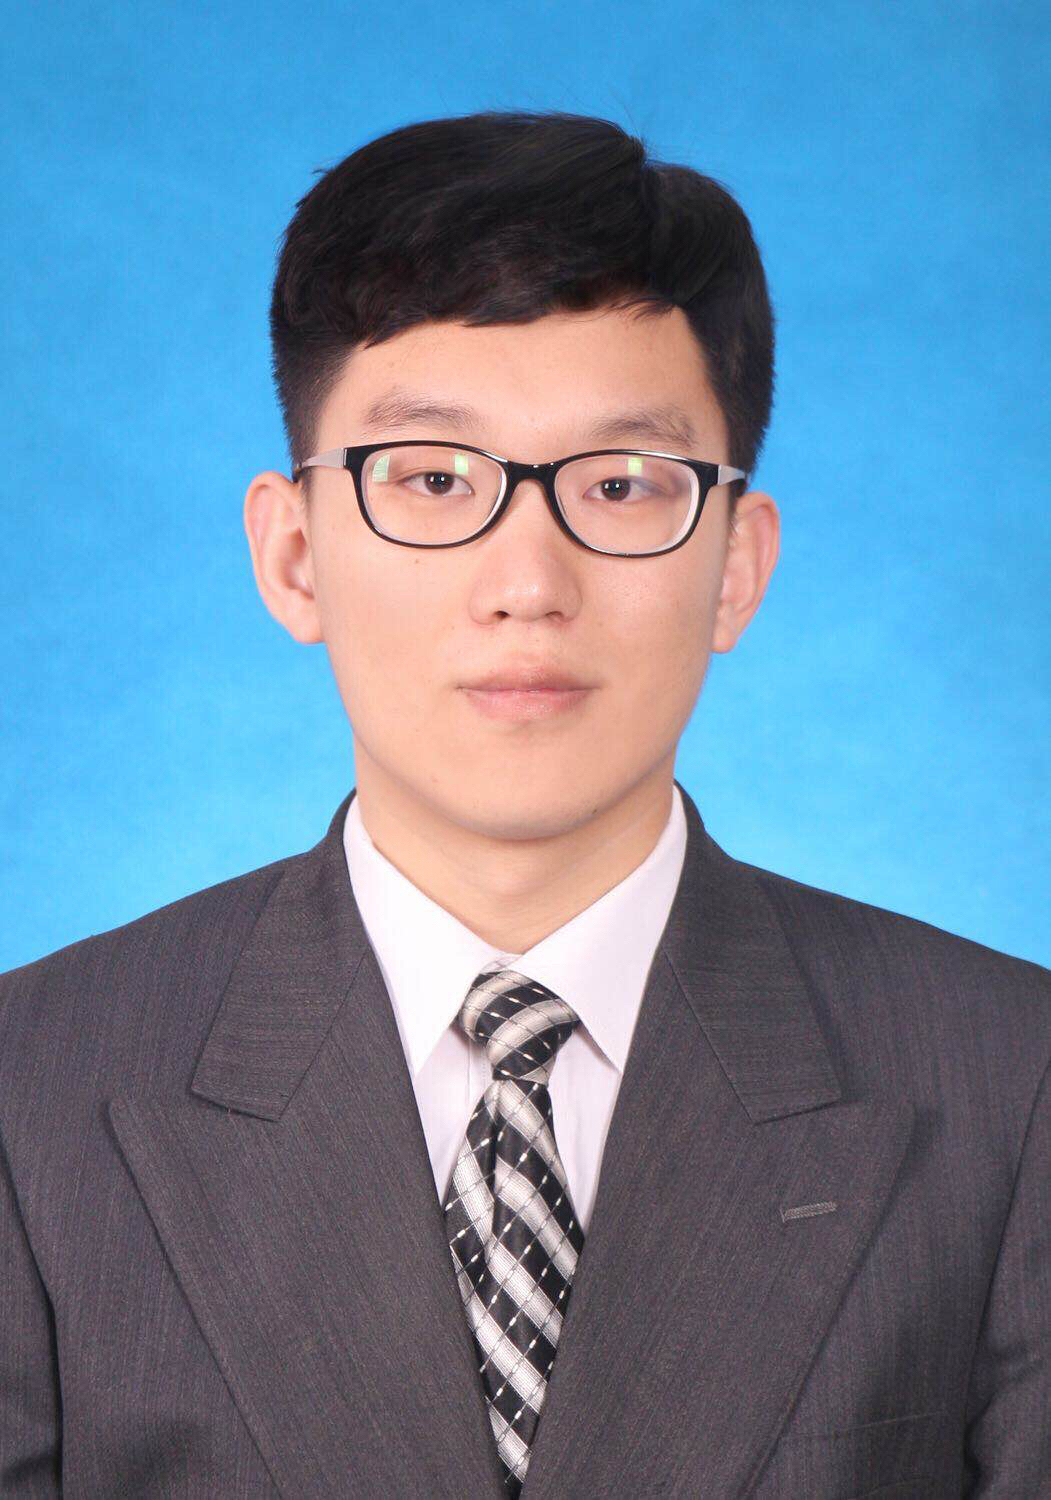
\includegraphics[width=0.19\textwidth]{pic.jpg}
\end{wrapfigure}
\section{基本信息}
\begin{tabular}{rl}
  \textsc{生日:} & 1993.12.03 \\
  \textsc{籍贯:} & 河南省鹤壁市 \\
  \textsc{地址:}   &  上海市闵行区东川路800号上海交通大学\\
  \textsc{手机:}     & 18818272991\\
  \textsc{邮箱:}     & \href{mailto:18818272991@163.com}{18818272991@163.com}\\
  \textsc{博客:}     & \href{https://zzsean.github.io}{https://zzsean.github.io}\\
\end{tabular}



%Section: Education
\section{学习经历}
\begin{tabular}{rl}	
  \textsc{2012.9 - } & 本科, \textbf{上海交通大学}, \textbf{电子信息与电气工程学院, 测控技术与仪器专业}\\
  \textsc{2016.7} & 并以专业第一的成绩得到研究生保送资格\\
& 主修课程: 模拟电路, 数字电路, 数据结构, c语言程序设计, python程序设计\\&\\
 \textsc{2016.9  } & 硕士研究生, \textbf{上海交通大学}, \textbf{电子信息与电气工程学院, 仪器科学与技术专业}\\
& 主修课程: 高级数字信号处理, 微弱信号检测, 视觉检测\\&\\
 \textsc{2017.10 - 11} & Coursera, Machine Learning课程, \textbf{最终成绩: 95.3/100}\\
& 学习并掌握了传统机器学习的相关原理和算法,如决策树, KNN, LR, SVM\\
& 等, 熟知其推导过程及相应的代码实现\\&\\
 \textsc{2017.11 - } & Coursera, Deep Learning课程\\
 \textsc{2018.1} & 斯坦福大学公开课, CS231n课程\\
& 学习并掌握了深度学习的相关原理和算法,如CNN, RNN, LSTM, GAN\\
& 等, 熟知其推导过程及相应的代码实现, 并能对相关论文中的算法进行复现,\\
& 学习使用Tensorflow, 熟悉深度学习算法实现的编程框架以及调参和优化\\
& 的思路和方法, 以及常用的深度神经网络模型等\\
\end{tabular}

%Section: Work Experience at the top
\section{开源项目}
\begin{tabular}{r|p{11cm}}
 \textsc{2017.9} & Handwritten Digits Recognition(手写数字识别) \\&\footnotesize{接触到的第一个,也是入门的深度学习开发项目. 整个项目使用Python编写, 选取了MNIST数据集, 对最简单的二维图像使用神经网络进行训练, 并通过改变神经网络的结构, 调整其中的参数, 深入理解了神经网络的原理, 并且不断地提高网络识别的准确度.}\\\multicolumn{2}{c}{} \\
 \textsc{2017.11} & Style Transfer(图像风格迁移)\\&\footnotesize{源论文: Leon A. Gatys et al. A Neural Algorithm of Artistic Style.}\\&\footnotesize{该项目使用Python编写, 并使用Tensorflow加以实现. 通过论文中给出的思路, 复现的重点在于对两种代价函数的计算, 其中又以风格代价函数为难点, 这一难点需要通过协方差矩阵来解决. 图片采用CNN的方式进行处理, 在这个过程中通过对不同网络的选取和参数的调整, 最终将论文中的结果较好的复现. }\\\multicolumn{2}{c}{} \\
 \textsc{2017.12} & Image Caption and Description(图像内容获取和描述)\\&\footnotesize{源论文: Kelvin Xu et al. Show, Attend and Tell: Neural Image Caption
Generation with Visual Attention.}\\&\footnotesize{该项目采用微软的COCO为数据集, 训练的过程分为两部: 编码和译码. 编码的过程是通过CNN对图像进行特征提取并输入. 译码的过程是通过RNN/LSTM训练生成对图片内容的文字描述.  }\\\multicolumn{2}{c}{} \\
\textsc{2018.2} & Generative Adversarial Networks(GAN, 生成对抗网络)\\&\footnotesize{源论文: Ian J. Goodfellow. Generative Adversarial Nets.}\\&\footnotesize{GAN可以用来生成质量很高的图片. 根据论文中所描述的原理, 实现GAN的根本就是生成器与判别器之间的博弈.这个项目中还是使用了Tensorflow来实现, 生成的是手写数字图片. 根据不同论文中描述的不同卷积神经网络结构或者代价函数实现了若干不同的GAN, 并比较了结果的优劣.}
\end{tabular}

%Section: Work Experience at the top
\section{科研经历}
\begin{tabular}{r|p{11cm}}
 \emph{目前} & 电子根尖测定仪 \\&\footnotesize{电子根尖测定仪的设计研究和改进为研究生阶段的主要课题,主要包括电路的设计,嵌入式程序的编写,数据的处理等, 主要涉及的是C语言和MATLAB. 以及针对目前电子根测仪在实际应用中出现的问题进行改善,期望将机器学习应用其中,从而改善测量的准确度.}\\\multicolumn{2}{c}{} \\
 \textsc{2016.1 - 6} & 主动降噪耳机控制系统 \\&\footnotesize{此研究课题通过主动噪声控制,利用LMS(最小均方算法)自适应算法,以Labview为基础搭建一个主动降噪耳机系统,通过MATLAB进行离线数据验证,成功实现耳机内的主动降噪.}\\\multicolumn{2}{c}{} \\
\textsc{2015.7} & 腕带式跌倒警报装置\\&\footnotesize{此课题中主要针对MPU6050传感器和相关判定跌倒算法进行学习,深入对STM32嵌入式编程的学习,包括数据的存储和文件读写,如串口通讯及FIFO等, 以及GPS的相关功能实现.}
\end{tabular}

%Section: Scholarships and additional info
\section{获奖经历\&证书}
\begin{tabular}{rl}
 \textsc{2014}  & 上海交通大学优秀奖学金B等\\
& "E + H" 专项奖学金\\
 \textsc{2015} & 上海交通大学优秀奖学金B等\\
& Java三级证书\\
 \textsc{2016} & 上海交通大学2016届优秀毕业生\\
\end{tabular}

%Section: Languages
\section{语言能力}
\begin{tabular}{rl}
英语: CET6 : 535, 可以流利的阅读英文文献并用英语交流\\
\end{tabular}

\section{计算机能力}
\begin{tabular}{rl}
 编程语言:& Python, ~~C\&C++, ~~Java, ~~MySQL \\
 编程工具:& MATLAB, ~~Labview, ~~Tensorflow, ~~{\fb \LaTeX}\setmainfont[SmallCapsFont=Fontin-SmallCaps.otf]{Fontin.otf}\\
 操作系统:& LINUX \\
 其他: & Office工具\\
\end{tabular}

\section{兴趣爱好}
足球~~游泳~~音乐~~电影


\end{document}
